%\begin{figure*}[]
%  \begin{adjustwidth}{-0.6cm}{}
%	\centering
%	\subfloat[Heavy hitter flows]{
%		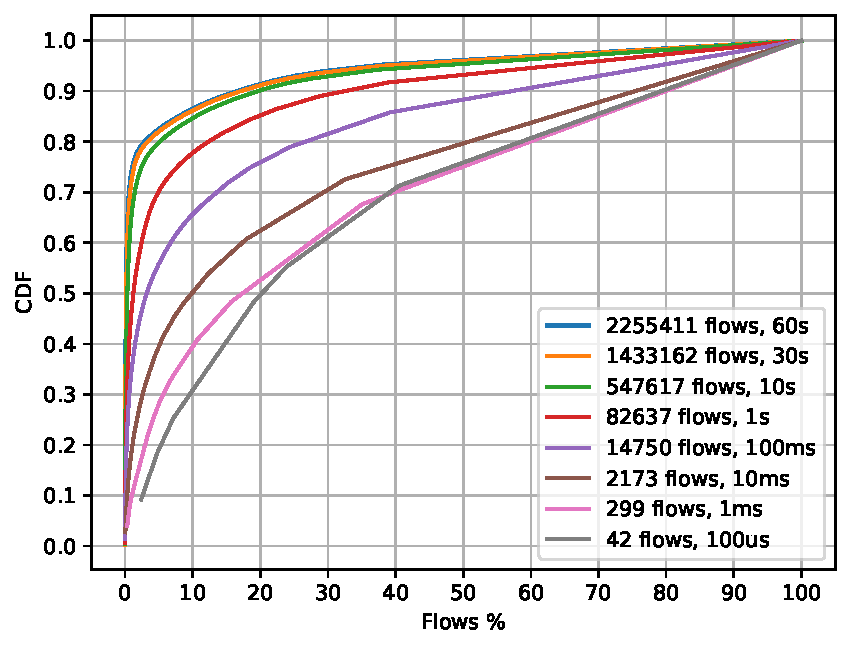
\includegraphics[width=0.26\textwidth]{fig_cdf_pkt.pdf}
%		\label{fig:cdf_pkt}
%	}%\qquad
%	\subfloat[Size-weighted heavy hitter flows]{
%		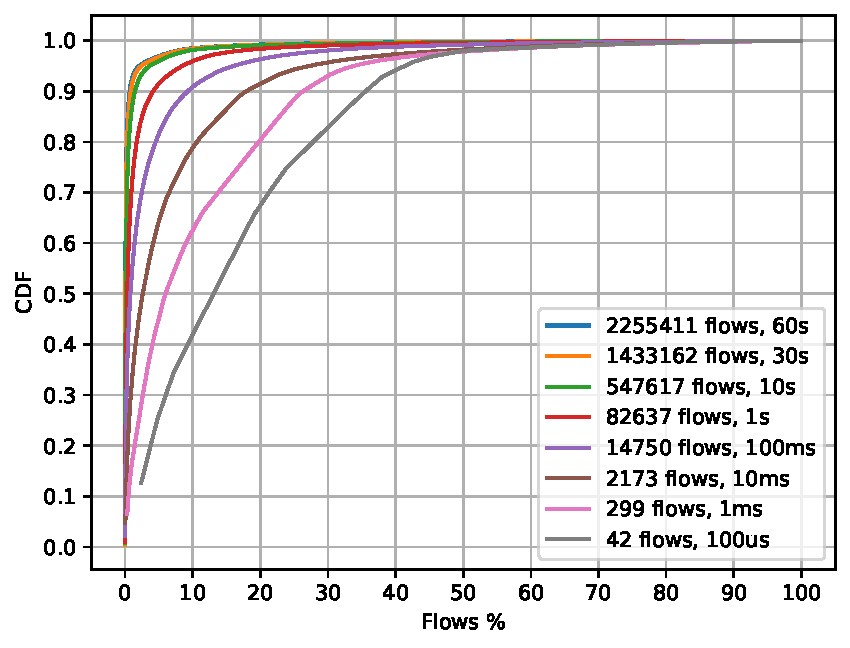
\includegraphics[width=0.26\textwidth]{fig_cdf.pdf}
%		\label{fig:cdf}
%	}%\\
%	\subfloat[Flow duration]{
%		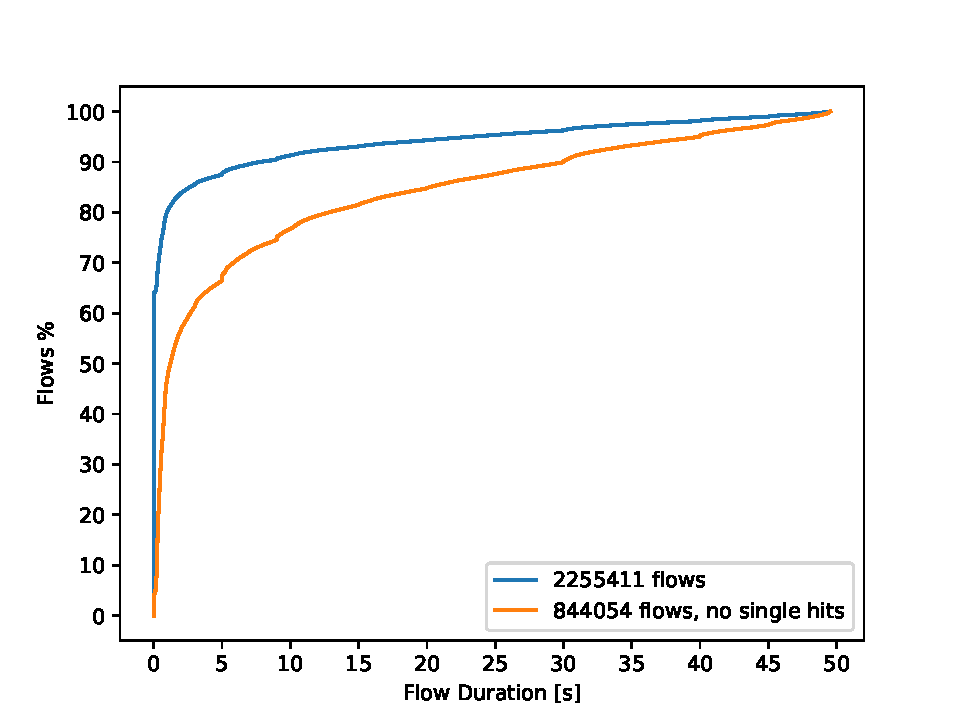
\includegraphics[width=0.26\textwidth]{fig_duration.pdf}
%		\label{fig:flow_duration}
%	}%\qquad
%	\subfloat[Average flow size]{
%		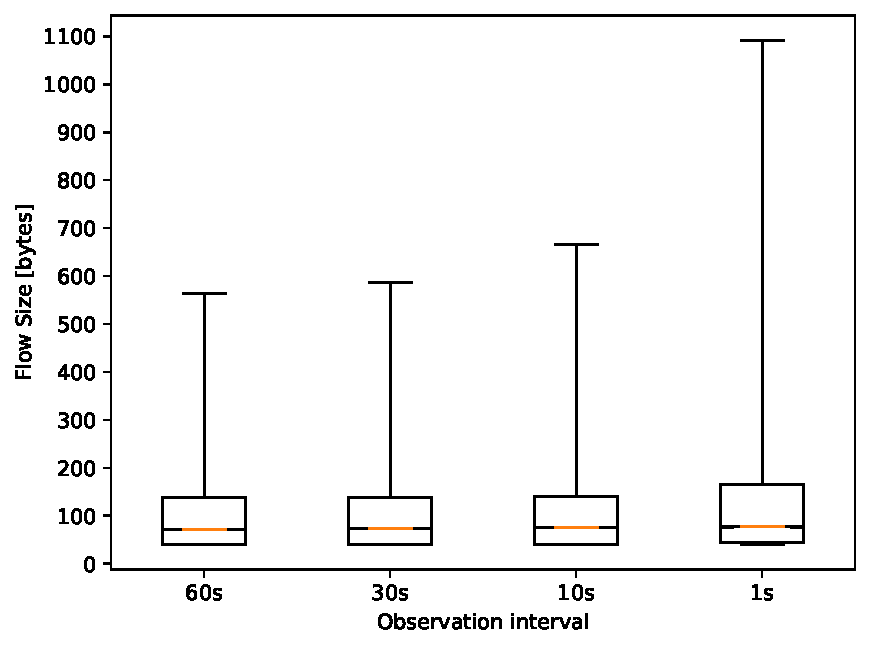
\includegraphics[width=0.26\textwidth]{fig_avg_flow_size.pdf}
%		\label{fig:flow_size}
%	}
%	\caption{CAIDA trace summary}
%	\label{fig:traces}
%	\end{adjustwidth}
%\end{figure*}

%\begin{figure*}[]
%	%	\begin{adjustwidth}{-0.6cm}{}
%	\centering
%	\subfloat[Heavy hitter flows]{
%		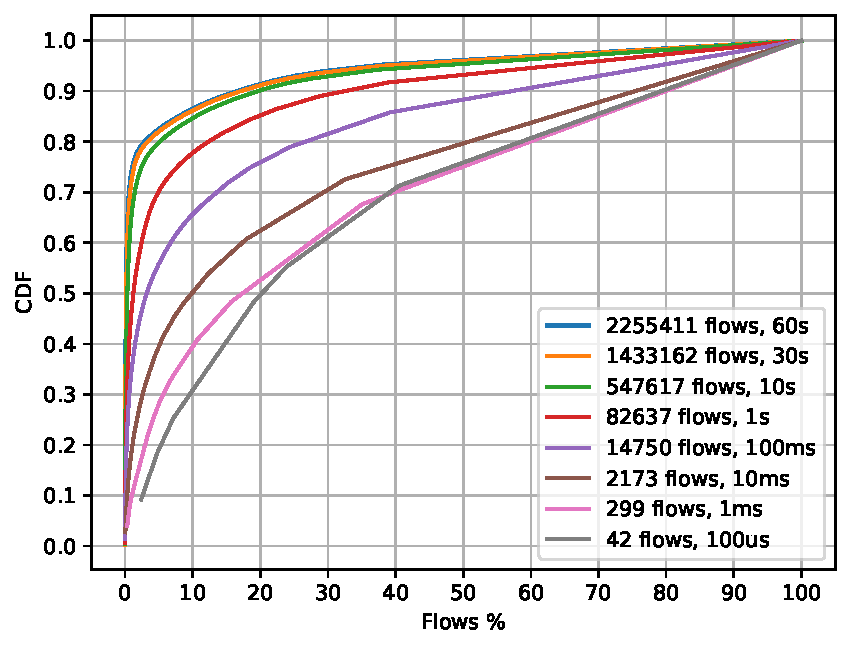
\includegraphics[width=0.4\textwidth]{fig_cdf_pkt.pdf}
%		\label{fig:cdf_pkt}
%	}\qquad
%	\subfloat[Size-weighted heavy hitter flows]{
%		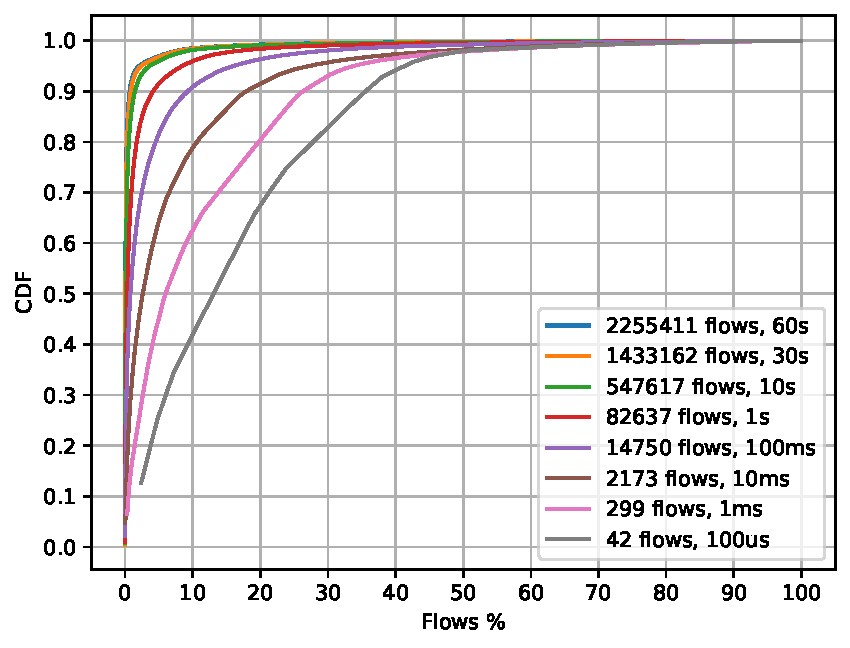
\includegraphics[width=0.4\textwidth]{fig_cdf.pdf}
%		\label{fig:cdf}
%	}\\
%	\subfloat[Flow duration]{
%		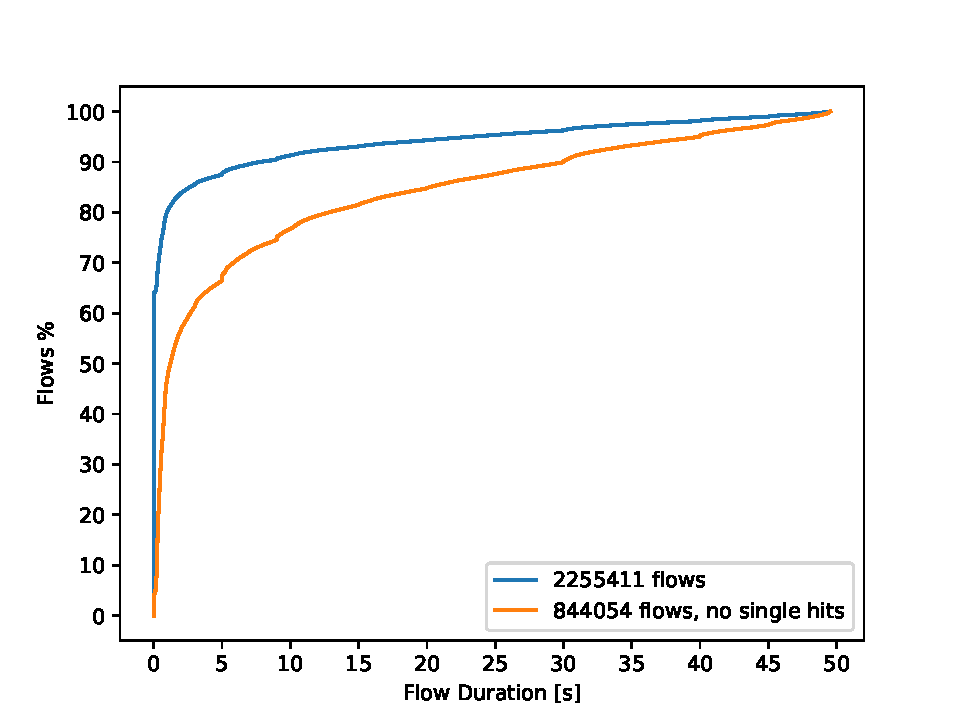
\includegraphics[width=0.4\textwidth]{fig_duration.pdf}
%		\label{fig:flow_duration}
%	}\qquad
%	\subfloat[Average flow size]{
%		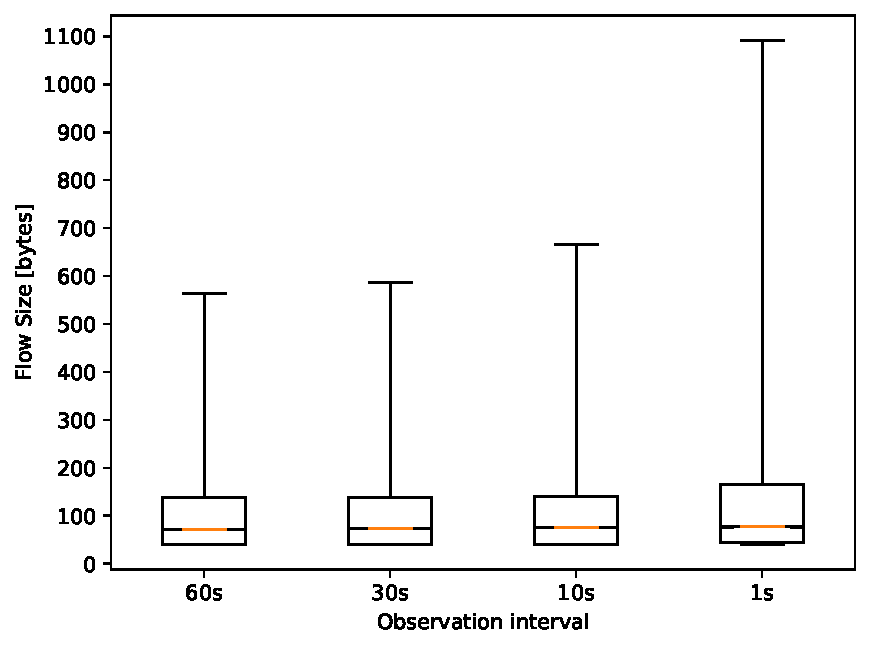
\includegraphics[width=0.4\textwidth]{fig_avg_flow_size.pdf}
%		\label{fig:flow_size}
%	}
%	\caption{CAIDA trace summary}
%	\label{fig:traces}
%	%	\end{adjustwidth}
%\end{figure*}


\section{Background}\label{sec:back}
This works proposes "infinitely" extending memory for high performance heterogeneous programmable dataplanes.
This is done by employing a cache hierarchy supported by network-aware cache policies.
This section first recaps traditional cache policies. 
Then, we review the constraints of current programmable dataplanes.

\subsection{Cache Replacement Algorithms}
\textbf{OPT}~---~The optimal (OPT) cache replacement policy~\cite{Belady:66} is an oracle algorithm that relies on knowing the future traffic behavior.
OPT uses this information to replace data that is further referenced in time.
Due to that, OPT is not realistically implementable and it is commonly used to evaluate cache performance since it sets an upper performance bound for realistic caching systems.

\textbf{Random}~---~Random or pseudo-random cache replacement policies use a stochastic random function to select a victim for eviction.
Pseudo-random cache policy has been widely adopted in ARM-based processors.
In random policies, no history on cache misses/hits nor cache access frequency is required.
The efficiency of a random policy is directly related to the quality of its random generator function.

\textbf{LRU}~---~The LRU cache replacement policy evicts the most ancient cache entry in case of a cache miss.
A possible LRU implementation uses a timestamp tag to sort cache entries by recency.%, as in Algorithm~\ref{algo:lru}.

%\begin{algorithm}[]
%	\caption{LRU policy}
%	\label{algo:lru}
%	\SetInd{0.1em}{.9em}
%	\SetAlgoLined
%	\footnotesize
%	\SetKwProg{procedure}{Procedure}{}{end}
%	\SetKwFunction{minTimestampEntry}{minTimestampEntry}
%	\SetKwFunction{findEntry}{findEntry}
%	\SetKwFunction{lruPolicy}{lruPolicy}
%	\SetKwInOut{Input}{input}
%	\SetKw{In}{in}%
%	\SetKw{Not}{not}%
%	\SetKw{Or}{or}%
%	\SetKw{Continue}{continue}%
%	\SetKw{True}{true}%
%	\Input{Cache memory: list of $\langle$\texttt{entry, timestamp}$\rangle$ pairs}
%	\Input{Possible cache entry}
%	\Input{Packet timestamp}
%	\procedure{\lruPolicy{cache, possible\_entry, current\_timestamp}}{
%		\If(\hfill\tcp*[h]{Cache hit}){possible\_entry \In cache}{
%			entry\_found =  \findEntry{cache, possible\_entry}\hfill\tcp{Hit pointer}
%			entry\_found$\rightarrow$timestamp  = current\_timestamp
%		}
%		\Else(\hfill\tcp*[h]{Cache Miss}){
%			victim = \minTimestampEntry{cache}\hfill\tcp{Victim pointer}			
%			*victim = $\langle$possible\_entry, current\_timestamp$\rangle$
%		}
%	}
%\end{algorithm}

\textbf{LFU}~---~Contrarily to LRU, LFU uses hit frequency rather than the access time to evict entries.
LFU uses a frequency counter to sort cache entries by frequency.
In case of a hit, the frequency counter is incremented.
Otherwise, the cache entry with the lowest frequency is chosen for eviction.%, as in Algorithm~\ref{algo:lfu}.
%
%\begin{algorithm}[]
%	\caption{LFU policy}
%	\label{algo:lfu}
%	\SetInd{0.1em}{.9em}
%	\SetAlgoLined
%	\footnotesize
%	\SetKwProg{procedure}{Procedure}{}{end}
%	\SetKwFunction{lfuPolicy}{lfuPolicy}
%	\SetKwFunction{findEntry}{findEntry}
%	\SetKwFunction{minFrequencyEntry}{minFrequencyEntry}
%	\SetKwInOut{Input}{input}
%	\SetKw{In}{in}%
%	\SetKw{Not}{not}%
%	\SetKw{Or}{or}%
%	\SetKw{Continue}{continue}%
%	\SetKw{True}{true}%
%	\Input{Cache memory: list of $\langle$\texttt{entry, counter}$\rangle$ pairs}
%	\Input{Possible cache entry}
%	\procedure{\lfuPolicy{cache, possible\_entry}}{
%		\If(\hfill\tcp*[h]{Cache hit}){possible\_entry \In cache}{
%			entry\_found = \findEntry{cache, possible\_entry}\hfill\tcp{Hit pointer}
%			entry\_found$\rightarrow$counter  += 1
%		}
%		\Else(\hfill\tcp*[h]{Cache miss}){
%			victim =  \minFrequencyEntry{cache}\hfill\tcp{Victim pointer}
%			*victim = $\langle$possible\_entry, 1$\rangle$
%		}
%	}
%\end{algorithm}


\subsection{Constraints of Programmable Dataplanes}\label{sec:constraints}

Single-chip homogeneous programmable dataplanes expose a clear trade-off on performance and memory resources.

State-of-the-art PISA-based programmable ASIC switches process packets at multi-terabit rates.
However, these switches have no more than a few hundreds of \SI{}{\mega\byte} of internal memory which is shared between lookup operations and user-defined stateful processing (e.g. metering, load-balancing).
Moreover, as these devices need to guarantee a very low fixed processing latency, programmers are not allowed to express loops or recursion that cannot be unrolled throughout physical pipeline stages.
Indeed, neither loops nor recursion is part of the P4 semantics.

On current programmable dataplanes, forwarding rules are installed by an external x86-like host CPU as they do not yet support table updates in the data plane.
Hence, there is no consensus w.r.t the maximum achieved match table update rate as many factors can influence it.
\citeauthor{Jin:2017} have reported an update rate in the order of \SI{10}{\kilo\update/\second}.
A first impacting factor is the host CPU load in which we have little control.
The match type also contributes to the update rate.
In our work, we are only interested in the exact match (EM) rule caching. 
EM tables are typically implemented as Cuckoo hash tables~\cite{Kirsch:2009,Bosshart:14}.
Cuckoo hash tables recursively move entries across hash tables to solve hash collisions when inserting a new table entry.
As the table load factor increases, several entries may be relocated which effectively decreases update rate.
Finally, the key and action sizes also impact the update rate.

The aforementioned constraints limit the feasibility of online cache policy algorithms.
Both LRU and LFU require extra information to select cache victims which increase memory usage.
Also, these cache policies require large data sorting, which is difficult to implement (if possible) in programmable PISA switches.
Finally, the match table update rate may sacrifice the reaction time of caching algorithms.

\section{Learning from the Traffic}\label{sec:traffic}

Network traffic has been observed to follow a Zipf distribution as few network flows account for most of the whole network traffic~\cite{Sarrar:2012, Jin:2017}.

In our study, we conducted experiments to determine the traffic characteristics of an up-to-date real-world data center trace.
We replayed a CAIDA network trace extracted from an IXP in a data center in New York dated from January 2019~\cite{caida:19}.
The analysed trace is 1 minute long monitoring $\sim$\SI{30}{\mega\nothing} packets in a full-duplex \SI{40}{\giga\bit/\second} Ethernet link connecting New York and S\~ao Paulo/Brazil.
A similar analysis was done by~\citeauthor{Spang:19} to estimate the number of TCP/IP flows~\cite{Spang:19}.

Figure~\ref{fig:traces} summarizes our observations.
In our analysis, we defined flow as being a unique five-tuple $\langle$~SrcIP, DstIP, protocol, SrcPort, DstPort~$\rangle$\footnote{We consider IPv4, IPv6, UDP, and TCP in our five-tuple definition.} connection.

\textbf{Heavy hitters}~---~As shown in Figure~\ref{fig:cdf_pkt} and Figure~\ref{fig:cdf}, the Zipf distribution characteristic is still present in current network traffic.
Both figures present the CDF, in terms of packet hits and byte hits, for several observation intervals, ranging from \SI{100}{\micro\second} to \SI{60}{\second}.
Although both curves are Zipfian-like, the exponent that characterizes the distributions in Figure~\ref{fig:cdf} is higher.
For all observation intervals longer than \SI{100}{\milli\second}, fewer than 10\% of the flows dominate more than 90\% of the traffic.
For shorter intervals, the Zipf dominance is still present although more skewed.

\textbf{Flow duration}~---~Figure~\ref{fig:flow_duration} presents the flow duration time.
The blue curve is dominated (60\%) by single packet flows.
Single packet flows are represented with a flow duration of zero seconds.
Short-lived flows dominate the trace with $\sim$90\% of all flows lasting less than 5 seconds.
The orange curve in Figure~\ref{fig:flow_duration} illustrates the duration of flows with multiple hits in the trace.
Still, short-lived flows dominate the trace with $\sim$50\% lasting less than 1 second.% in the trace.

\textbf{Flow size}~---~Figure~\ref{fig:flow_size} presents the average flow size for four statistically representative observation intervals.
For all four measures, the first quartile, the median, and the third quartile are very similar.
On average, small flows ($\sim$100 bytes) dominate the trace with 75\% of the flows being no larger than 150 bytes.
\begin{algorithm}[t]
	\caption{WLFU policy}
	\label{algo:wlfu}
	\SetInd{0.1em}{.9em}
	\SetAlgoLined
	\footnotesize
	\SetKwProg{procedure}{Procedure}{}{end}
	\SetKwFunction{wlfuPolicy}{wlfuPolicy}
	\SetKwFunction{findEntry}{findEntry}
	\SetKwFunction{minFrequencyEntry}{minFrequencyEntry}
	\SetKwInOut{Input}{input}
	\SetKw{In}{in}%
	\SetKw{Not}{not}%
	\SetKw{Or}{or}%
	\SetKw{Continue}{continue}%
	\SetKw{True}{true}%
	\Input{Cache memory: list of $\langle$\texttt{entry, counter}$\rangle$ pairs}
	\Input{Possible cache entry}
	\Input{Packet Size}
	\procedure{\wlfuPolicy{cache, possible\_entry, pkt\_size}}{
		\If(\hfill\tcp*[h]{Cache hit}){possible\_entry \In cache}{
			entry\_found =  \findEntry{cache, possible\_entry}\hfill\tcp{Hit pointer}
			entry\_found$\rightarrow$counter  += pkt\_size\hfill\tcp{Increment size counter}
		}
		\Else(\tcp*[h]{Cache miss}){
			victim =  \minFrequencyEntry{cache}\hfill\tcp{Victim pointer}
			*victim = $\langle$possible\_entry, pkt\_size$\rangle$
		}
	}
\end{algorithm}
According to our experiments, the expected Zipf distribution characteristic of network traffic is still present in current data center traffic.
Such characteristic favors flow caching in memory scarce programmable dataplanes.
However, the heavy-hitter analyses show that transmitted byte-based heavy hitters are more dominant than packet-based ones.
Thus, frequency-based cache policies (e.g. LFU) must consider the actual packet size in their frequency counters.
In addition to that, we notice that short-lived flows dominate the trace.
Therefore, the chosen cache policy algorithm needs a fast reaction time to quickly adapt to traffic changes.
Besides, such temporal traffic characteristic possibly favors time-aware cache policies (e.g. LRU).

\section{Traffic-aware Cache Policies}\label{sec:policies}
As traditional cache replacement positions may not be suitable in network scenarios, in this section we introduce network-aware cache policies.
Based on the real traffic analysis, we first present cache eviction policies.
Then, we present cache promotion policies aiming at maximizing cache performance.

\subsection{Cache Eviction}\label{sec:evi}

\textbf{WLFU}~---~\textit{Vanilla} implementations of LFU perform poorly with real-world network traces~\cite{Kim:09}.
\textit{Vanilla} LFU considers all cache hits with equal weight, which is not realistic in network communications because larger packets result in greater network efficiency compared to small ones.
Thus, Weighted LFU (WLFU) leverages LFU by considering the packet size in its frequency counters.
A possible implementation of WLFU is illustrated in Algorithm~\ref{algo:wlfu}.
Note that as frequency counters are always increasing, periodically flushes (omitted in the pseudocode) are required.
%\begin{algorithm}[t]
%\caption{WLFU policy}
%\label{algo:wlfu}
%\SetInd{0.1em}{.9em}
%\SetAlgoLined
%\footnotesize
%\SetKwProg{procedure}{Procedure}{}{end}
%\SetKwFunction{wlfuPolicy}{wlfuPolicy}
%\SetKwFunction{findEntry}{findEntry}
%\SetKwFunction{minFrequencyEntry}{minFrequencyEntry}
%\SetKwInOut{Input}{input}
%\SetKw{In}{in}%
%\SetKw{Not}{not}%
%\SetKw{Or}{or}%
%\SetKw{Continue}{continue}%
%\SetKw{True}{true}%
%\Input{Cache memory: list of $\langle$\texttt{entry, counter}$\rangle$ pairs}
%\Input{Possible cache entry}
%\Input{Packet Size}
%\procedure{\wlfuPolicy{cache, possible\_entry, pkt\_size}}{
%	\If(\hfill\tcp*[h]{Cache hit}){possible\_entry \In cache}{
%		entry\_found =  \findEntry{cache, possible\_entry}\hfill\tcp{Hit pointer}
%		entry\_found$\rightarrow$counter  += pkt\_size\hfill\tcp{Increment size counter}
%	}
%	\Else(\tcp*[h]{Cache miss}){
%		victim =  \minFrequencyEntry{cache}\hfill\tcp{Victim pointer}
%		*victim = $\langle$possible\_entry, pkt\_size$\rangle$
%	}
%}
%\end{algorithm}

\textbf{OLFU}~---~Optmistic LFU (OLFU) is a proposition to overcome the limitations of \textit{vanilla} LFU for flow caching.
OLFU is an LFU derivation that gives a chance for a cache promotion candidate to remain in cache regardless of its \textit{actual} hit frequency.
In OLFU, the cache policer behaves as the LFU in case of a cache hit.
Otherwise, instead of re-initializing the frequency counter, the new cache entry takes control of the victim's counter, as shown in Algorithm~\ref{algo:olfu} that omits the flushing logic.
\begin{algorithm}[t]
\caption{OLFU policy}
\label{algo:olfu}
\SetInd{0.1em}{.9em}
\SetAlgoLined
\footnotesize
\SetKwProg{procedure}{Procedure}{}{end}
\SetKwFunction{olfuPolicy}{olfuPolicy}
\SetKwFunction{findEntry}{findEntry}
\SetKwFunction{minFrequencyEntry}{minFrequencyEntry}
\SetKwInOut{Input}{input}
\SetKw{In}{in}%
\SetKw{Not}{not}%
\SetKw{Or}{or}%
\SetKw{Continue}{continue}%
\SetKw{True}{true}%
\Input{Cache memory: list of $\langle$\texttt{entry, counter}$\rangle$ pairs}
\Input{Possible cache entry}
\procedure{\olfuPolicy{cache, possible\_entry}}{
	\If(\hfill\tcp*[h]{Cache hit}){possible\_entry \In cache}{
		entry\_found =  \findEntry{cache, possible\_entry}\hfill\tcp{Hit pointer}
		entry\_found$\rightarrow$counter += 1
	}
	\Else(\hfill\tcp*[h]{Cache miss}){
		victim = \minFrequencyEntry{cache}\hfill\tcp{Victim pointer}
		*victim = $\langle$possible\_entry, victim$\rightarrow$counter + 1$\rangle$\hfill\tcp{Replace reusing current counter}
	}
}
\end{algorithm}

\textbf{OWLFU}~---~To optimize cache efficiency, OWLFU combines the OLFU and WLFU cache policies.
In case of a hit, OWLFU behaves as WLFU.
Otherwise, OWLFU modifies OLFU by incrementing the current packet size to the victim frequency counter, as in Algorithm~\ref{algo:owlfu}.
\begin{algorithm}[]
\caption{OWLFU policy}
\label{algo:owlfu}
\SetInd{0.1em}{.9em}
\SetAlgoLined
\footnotesize
\SetKwProg{procedure}{Procedure}{}{end}
\SetKwFunction{owlfuPolicy}{owlfuPolicy}
\SetKwFunction{findEntry}{findEntry}
\SetKwFunction{minFrequencyEntry}{minFrequencyEntry}
\SetKwInOut{Input}{input}
\SetKw{In}{in}%
\SetKw{Not}{not}%
\SetKw{Or}{or}%
\SetKw{Continue}{continue}%
\SetKw{True}{true}%
\Input{Cache memory: list of $\langle$\texttt{entry, counter}$\rangle$ pairs}
\Input{Possible cache entry}
\Input{Packet Size}
\procedure{\owlfuPolicy{cache, possible\_entry, pkt\_size}}{
	\If(\hfill\tcp*[h]{Cache hit}){possible\_entry \In cache}{
		entry\_found =  \findEntry{cache, possible\_entry}\hfill\tcp{Hit pointer}
		entry\_found$\rightarrow$counter  += pkt\_size\hfill\tcp{Increment size counter}
	}
	\Else(\hfill\tcp*[h]{Cache miss}){
		victim =  \minFrequencyEntry{cache}\hfill\tcp{Victim pointer}
		*victim = $\langle$possible\_entry, victim$\rightarrow$counter + pkt\_size$\rangle$\hfill\tcp{Replace reusing current size counter}
	}
}
\end{algorithm}

\begin{figure*}[]
	\centering
	\subfloat[Hit Ratio. $SF=1\times$]{
		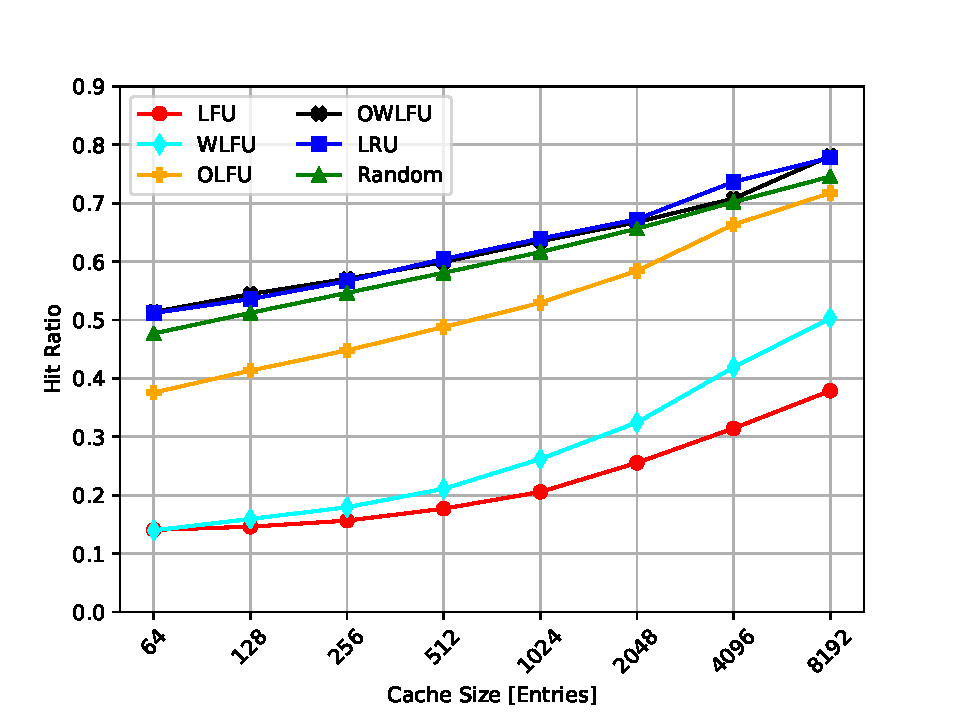
\includegraphics[width=0.33\textwidth]{../scripts/hit_ratio_sf1.pdf}
		\label{fig:hit_ratio_sf1}
	}
	\subfloat[Hit Ratio. $SF=10\times$]{
		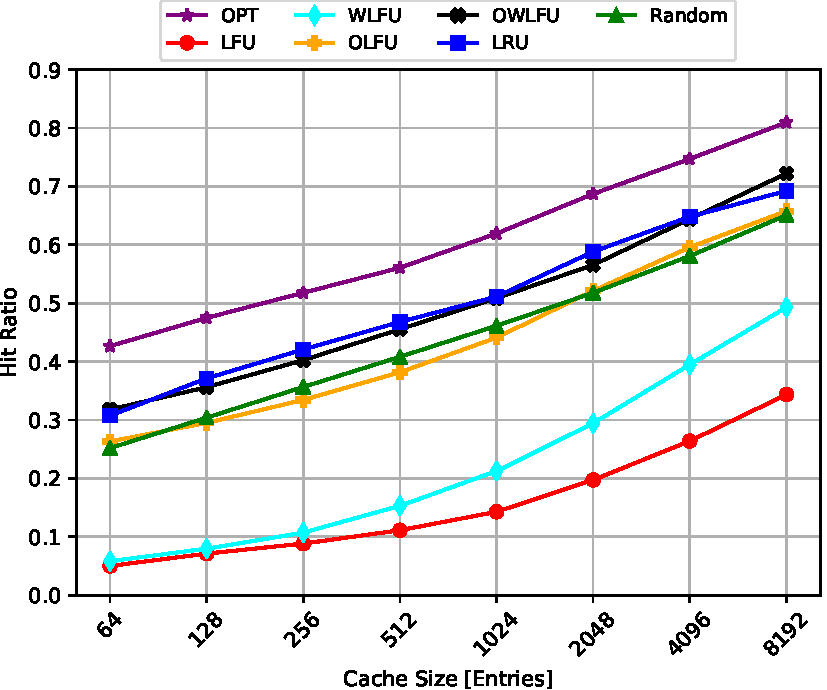
\includegraphics[width=0.33\textwidth]{../scripts/hit_ratio_sf10.pdf}
		\label{fig:hit_ratio_sf10}
	}
	\subfloat[Hit Ratio. $SF=100\times$]{
		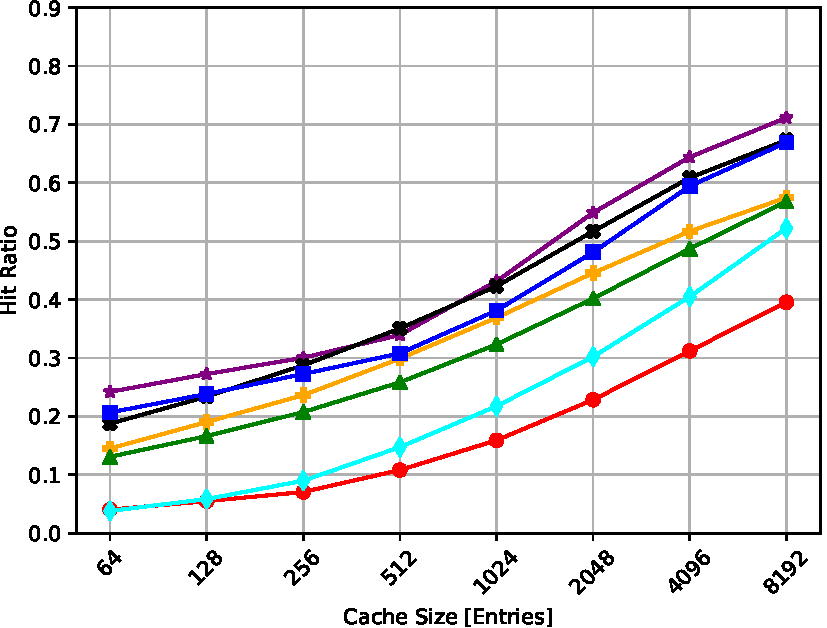
\includegraphics[width=0.33\textwidth]{../scripts/hit_ratio_sf100.pdf}
		\label{fig:hit_ratio_sf100}
	}\\
	\subfloat[Size Weighted Hit Ratio. $SF=1\times$]{
		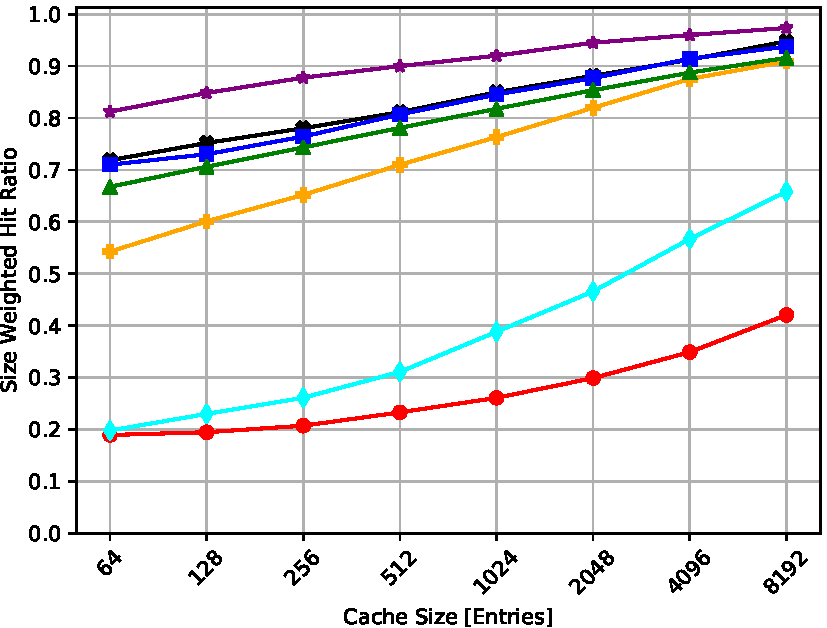
\includegraphics[width=0.33\textwidth]{../scripts/weighted_hit_ratio_sf1.pdf}
		\label{fig:weighted_hit_ratio_sf1}
	}
	\subfloat[Size Weighted Hit Ratio. $SF=10\times$]{
		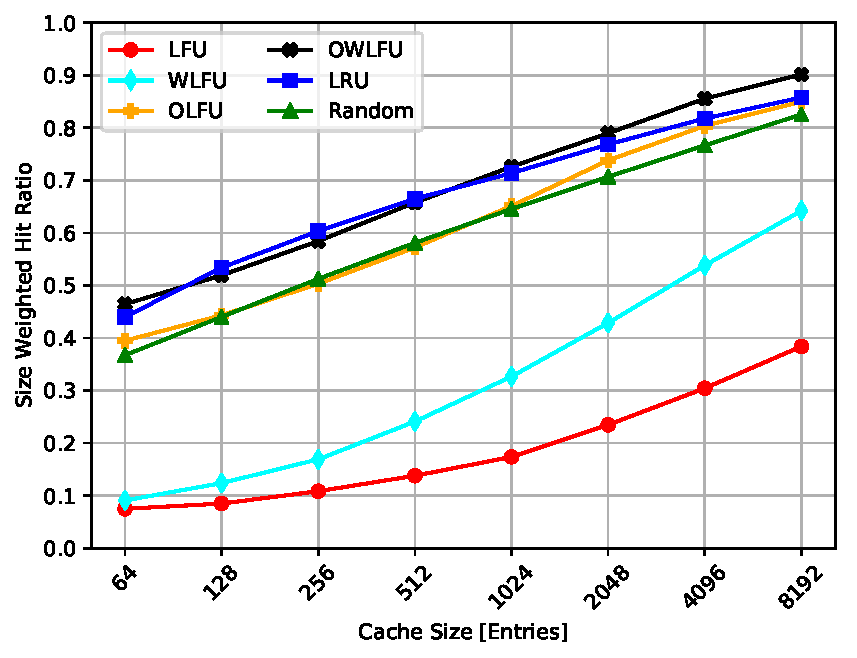
\includegraphics[width=0.33\textwidth]{../scripts/weighted_hit_ratio_sf10.pdf}
		\label{fig:weighted_hit_ratio_sf10}
	}
	\subfloat[Size Weighted Hit Ratio. $SF=100\times$]{
		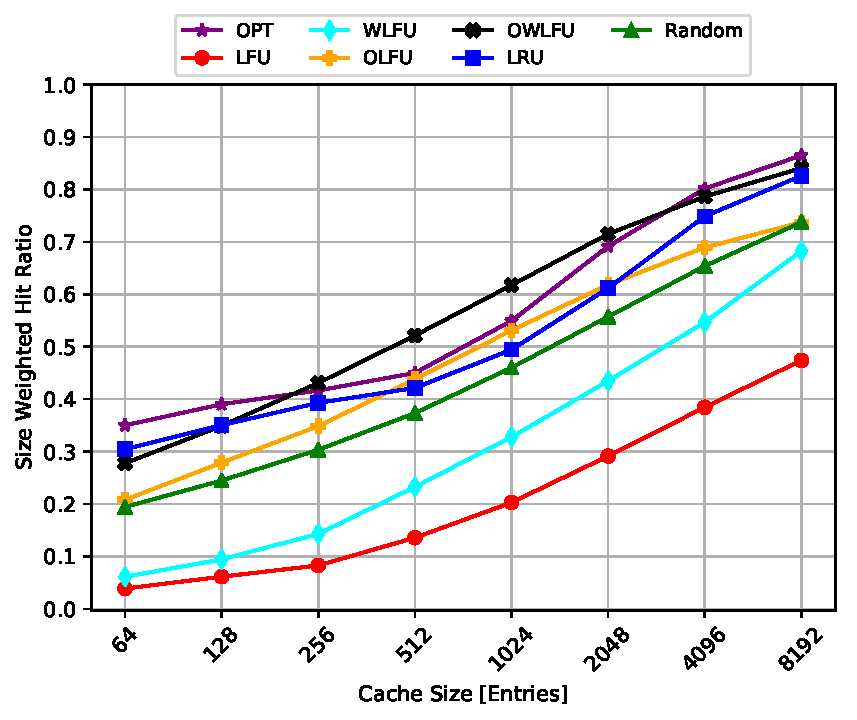
\includegraphics[width=0.33\textwidth]{../scripts/weighted_hit_ratio_sf100.pdf}
		\label{fig:weighted_hit_ratio_sf100}
	}
	\caption{Cache performance evaluation when no promotion policy implemented}
	\label{fig:hit_ratio}
\end{figure*}


\subsection{Cache Promotion}
Due to traffic dynamics and programmable dataplane constraints, heuristic cache promotion policies are required for flow caching.
Thus, we present two policies based on traffic observations.

\textbf{WMFU}~---~Heavy hitters are dominant in current data center traffic.
As a consequence, selecting heavy hitters that generate cache misses are potential candidates for cache promotion.
Thus, Weighted Most Frequently Used (WMFU) is a traffic-aware promotion policy derived from MFU.
In classic MFU, frequent items are tracked for cache eviction.
Hence, WMFU modifies MFU by considering the packet size in its frequency counters.
Missed flows with higher counters are thus marked for cache promotion.

\textbf{OWMFU}~---~Optimistic WMFU is the OWLFU counterparts presented in \S\ref{sec:evi}.
OWMFU optimistically speculates that frequent hitters will continue hitting soon after.
Similarly to WMFU, most frequent missed flows are selected for cache promotion.



\section{Evaluating Cache Performance}\label{sec:cache_results}
In this section, we present the simulation results for an HDP caching system.
Thus, we discuss the viability of such a caching system.
Finally, we discuss the limitations of our approach.

\subsection{Experimental Setup}
Table~\ref{tab:setup} presents the simulation parameters used to evaluate a two-level caching system as in Figure~\ref{fig:high_level_network}.
We simulated the cache performance by emulating different cache policer slowdown factor ($SF$).
Note, that for a two-level caching scheme, $SF$ also represents the cache policer reaction time.
As performance metrics, we reported the cache hit ratio and the traffic size weighted hit ratio.
%The term slowdown factor ($SF$) refers to the cache policer reaction time.
%The slowdown factor is relative to the cache speed, i.e., a slowdown of 10$\times$ means that the cache policer is 10$\times$ slower than cache access.
%The presented results were generated using the IXP New York to S\~ao Paulo data center trace~\cite{caida:19}.
The simulated traffic trace is the same as in~\S\ref{sec:traffic}.
To enable reproducibility, we open-sourced our codes\footnote{\url{https://github.com/engjefersonsantiago/Infinite_MT}.}.


\begin{table}[]
	\centering
	\caption{Experimental Parameters}
	\label{tab:setup}
	\begin{tabular}{l|l}
		\toprule
		\textbf{Parameter}       & \textbf{Value}   \\
		\midrule
		Eviction policy            & LRU, (O)(W)LFU, Random			    \\
		Promotion policy            & None, (O)WMFU			    \\
		Cache Size              & 64 to \SI{8}{\kilo\nothing} entries  \\
		Slowdown Factor         & 1$\times$, 10$\times$, 100$\times$        \\
		\bottomrule
	\end{tabular}
\end{table}

\subsection{Simulation Results}
Figure~\ref{fig:hit_ratio} presents the results for our experiments when no promotion policy is implemented.

As already reported in~\cite{Kim:09}, \textit{vanilla} LFU performs poorly with real-world network traffic.
Also, we confirmed the good performance of LRU-based policies with up-to-date data center traffic. 
The random policy achieves a relatively good cache performance considering the small overhead for implementing it.
Random policy hit ratio lags behind the classic LRU by no more than 10\%.

All modified versions of LFU significantly improve the cache performance compared to the \textit{vanilla} LFU.
WLFU observes a sharp increase in its hit ratio as the cache size increases.
OLFU observes a steady performance approaching the random hit ratio.
Indeed, OLFU introduces a pseudo-temporal variable to the LFU policy because it speculates that the promoted cache entry will be referenced soon after. 
Last, OWLFU performs best in almost all scenarios.
This is nonetheless expected since it combines the strengths of OLFU and WLFU.

%TODO: Check and run OPT simulations.
%TODO: Comment the SF effect.
Figure~\ref{fig:promo_fig} presents the impact of heuristic cache promotion. 
We evaluated two cache promotion policies: WMFU and OWMFU.
These policies were combined with three cache eviction policies: random, LRU, and OWLFU.
We fixed the cache size to \SI{8}{\kilo\nothing} entries and we ran simulations with $SF=10\times$ and $SF=100\times$ because heuristic cache promotion is only applicable when $SF>1\times$.
\begin{figure*}[]
	\centering
	\subfloat[Hit Ratio.]{
		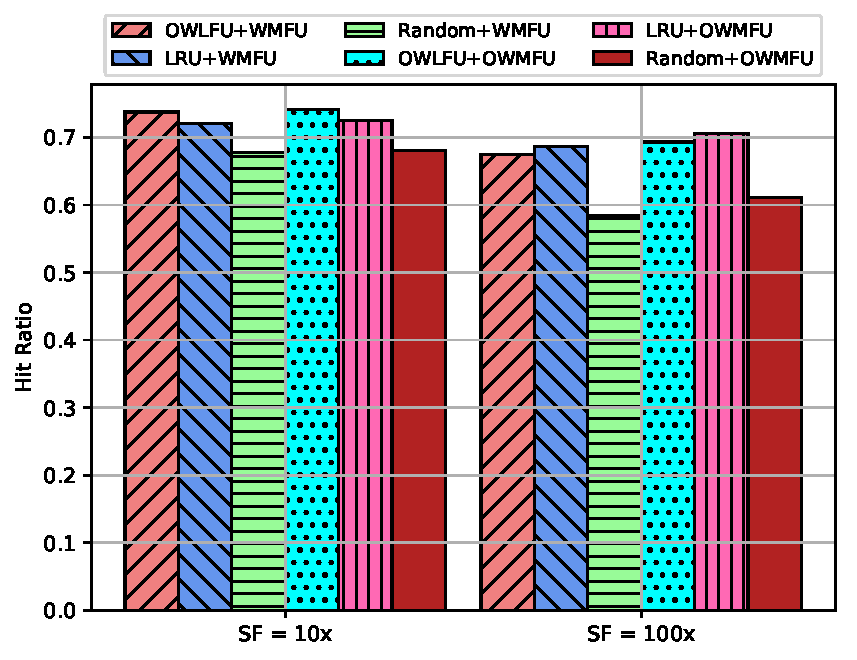
\includegraphics[width=0.43\textwidth]{../scripts/promo.pdf}
		\label{fig:promo}
	}\qquad
	\subfloat[Size Weighted Hit Ratio.]{
		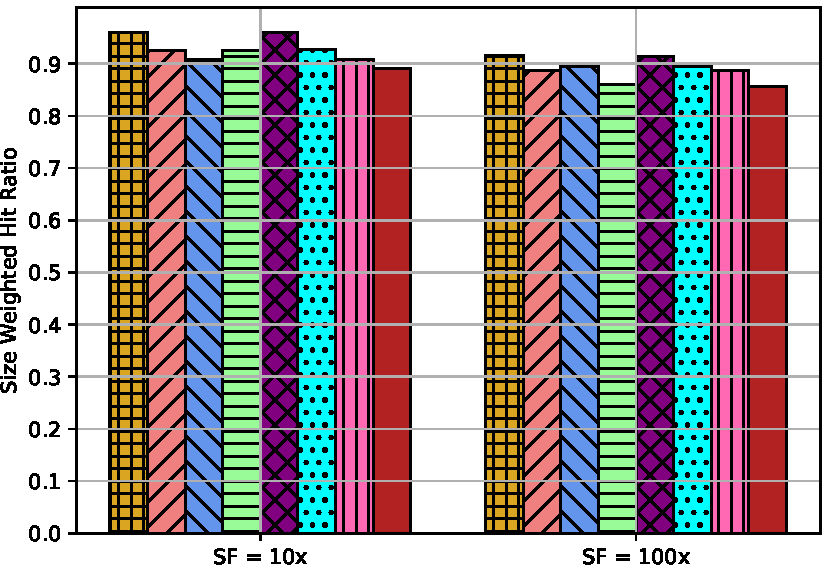
\includegraphics[width=0.43\textwidth]{../scripts/promo_weighted.pdf}
		\label{fig:promo_weighted}
	}
	\caption{Cache performance evaluation when promotion policies are implemented}
	\label{fig:promo_fig}
\end{figure*}

The simulation shows a noticeable increase (+10\%) in the cache hit ratio for when a random-based eviction policy is implemented.
Moreover, the results also suggest that there is no significant gain when LRU and LFU derivations are used.

\subsection{Discussions}

Although LRU and LFU derivations present the best simulation results, these cache policies may be difficult to implement in high-performance programmable dataplanes.
First, in terms of memory consumption, both replacement classes require $O(N)$ extra information to select cache victims.
This is undesirable because memory is scarce in network switches and must be reserved for profitable applications.
Second, both algorithms require sorting data either by frequency or time, a costly and non-scalable operation as it requires at least $O(N~log(N))$ comparisons with $O(log(N))$ time complexity.
Moreover, such parallel sorting would require N-port read memory, which is not available in current programmable dataplanes.
An alternative would be sorting the data in software, however, the increasing data rates of current programmable dataplanes make this infeasible.  

An alternative naive software approach for implementing LRU caches is using doubly-linked lists.
This approach is also infeasible in current programmable dataplanes.
The main reason is due to the feed-forward pipeline organization which prevents backpropagation of data from a stage $S_{i}$ to $S_{i-1}$.
Singly-linked lists could, however, be used for implementing an LRU cache.
The most recent element would be placed at the head of the list while other elements are moved towards the tail.
If the most recent element is already in the list, the data moving stops at its position, otherwise, it continues down to the tail.
Such implementation is possible in programmable dataplanes, however, it is still infeasible due to the limited number of pipeline stages (commonly fixed at 32 stages).
Multiple parallel singly-linked lists are possible but the scalability is as well limited.

Not surprisingly, the performance of random-based policies applied to caches with Zipfian access patterns approaches to classic (LRU) and novel (OWLFU) policies.
These results follow what has been reported in the literature~\cite{Gallo:2014}.
The simulation results show the cache hit ratio based on a random replacement policy is less than 10\% lower than LRU and OWLFU.
Moreover, implementing a random replacement policy in programmable dataplanes has no additional hardware cost as it may be implemented in software.

Contrary to LRU and LFU, implementing cache promotion policies in the data plane is viable.
MFU and its presented derivations can be considered as a subclass of the classic top-k hot items problem~\cite{Metwally:2005}.
Detecting top-k hot items have been already demonstrated in P4~\cite{Sivaraman:17} and Domino~\cite{SivaramanDomino:2016} targeting current programmable dataplanes with sublinear memory consumption.

Although we are mainly interested in the data plane aspects of match table caching, the control plane component also plays an important role.
Considering the constraints discussed in~\S\ref{sec:constraints}, the control plane ability in detecting and installing match table entries may expose a performance bottleneck, as reported by \citeauthor{Miao:2017} when designing a stateful load balancer~\cite{Miao:2017}.
\citeauthor{Miao:2017} have found that the software overhead was related to the CPU load for hash calculations, not in the PCIe CPU-switch communication.
However, a match table cache scheme has more stringent requirements in terms of match table update rate considering the observed flows lifetime.
Thus, CPU-switch communication may still have a significant impact on performance for heterogeneous flow caching as the different HDP components are likely to have mismatched communication interfaces.

\subsection{Limitations}\label{sec:method:limitations}

\textbf{Prefix shadowing}~---~In this work, we are interested in detecting possible candidates for flow migration in the data plane.
This is due to high-speed links in data center networks and the fast-changing nature of data center network traffic; therefore, a slow control plane interaction must be minimized.
However, candidates detection for flow migration in the data plane can only be precisely detected for exact match rules due to the shadowing effect in ternary and LPM rules.
For example, let us consider a case where a low priority LPM rule is frequently matched in a low cache level and would, therefore, be a candidate for flow migration.
Using our method, this rule is moved to a higher cache level as expected.
Now, a high priority rule belonging to the same prefix arriving at the HDP switch will match in the high cache level.
However, a specific rule installed in a lower cache level for the same prefix will be shadowed, leading thus to a possibly wrong forwarding decision.   
Such cache ambiguity is a known problem and it has been reported and addressed in earlier works~\cite{Degermark:1997, Katta:2014}.

\textbf{Simulator Limits}~---~The eviction and promotion cache policies evaluated in this work were fine-tuned based on an actual real-world data center network trace.
This analysis showed that the traffic followed a Zipf distribution.
Employing the caching strategy proposed in this work in other traffic scenarios has not yet been explored.
As a consequence, our methods and propositions may not be viable in different traffic distributions.

The performance analysis in this paper has considered only a 2-level cache.
However, an N-level cache can be generalized as an (N~$-$~1) independent 2-level caches.
Thus, the conducted 2-level cache performance investigation is relevant for setting an upper bound hit ratio analysis, even though we agree that a full caching system may expose other limitations, such as multi-level control plane interaction.

In our simulator, all table update metrics (communication, table insertion times, CPU load) are enveloped in a unified $SF$ metric.
Although $SF$ attempts to mimic performance gaps, in real hardware it may not be realistic.
For example, our simulator considers a perfect EM table disregarding \textit{actual} hardware implementations in which a single table insertion may trigger many table modifications, which increases CPU load and communication overhead.
Finally, our simulator does not support batching for either table insertion nor when gathering eviction/promotion policy counters.

